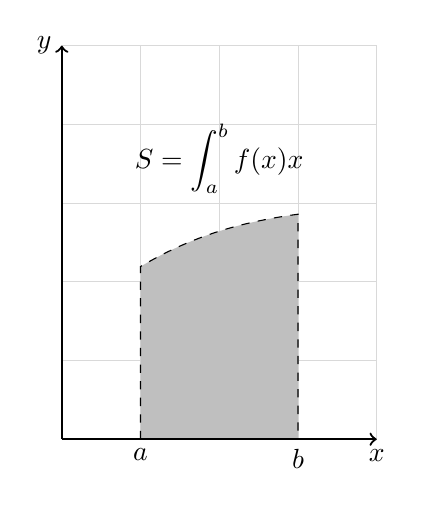
\begin{tikzpicture}
  \draw[very thin, gray!30, step = 1cm] (0, 0) grid (4, 5);
  \fill[lightgray, domain = 1 : 3, variable = \x]
    (1, 0)
    -- plot ({\x}, {3 / (1 + e^(-\x))})
    -- (3, 0)
    -- cycle;
  \draw[dashed, domain = 1 : 3, variable = \x]
    (1, 0)
    -- plot ({\x}, {3 / (1 + e^(-\x))})
    -- (3, 0);

  \draw[thick] [->] (0, 0) -- (4, 0) node[right, below] {\(x\)};
  \draw[thick] [->] (0, 0) -- (0, 5) node[above, left] {\(y\)};
  \draw node[above] at (2, 3) {\(\displaystyle
    S = \int_{a}^{b} f(x) \dd x
  \)};
  \draw node[below] at (1, 0) {\(a\)};
  \draw node[below] at (3, 0) {\(b\)};
\end{tikzpicture}
